
\documentclass{article}

\usepackage{pttyr_descriptions}

\begin{document}

\setlist{nolistsep}
\nointerlineskip
\par\noindent
\setlength{\parindent}{0pt}


\section*{Recurrent Networks}
\subsection*{\ttt{torch.nn.RNN}}
\prepostc{torch.nn.RNN(input\_size, hidden\_size, num\_layers=1,
nonlinearity=`tanh', bias=True, batch\_first=False, dropout=0,
bidirectional=False)(input, hidden)}{
  %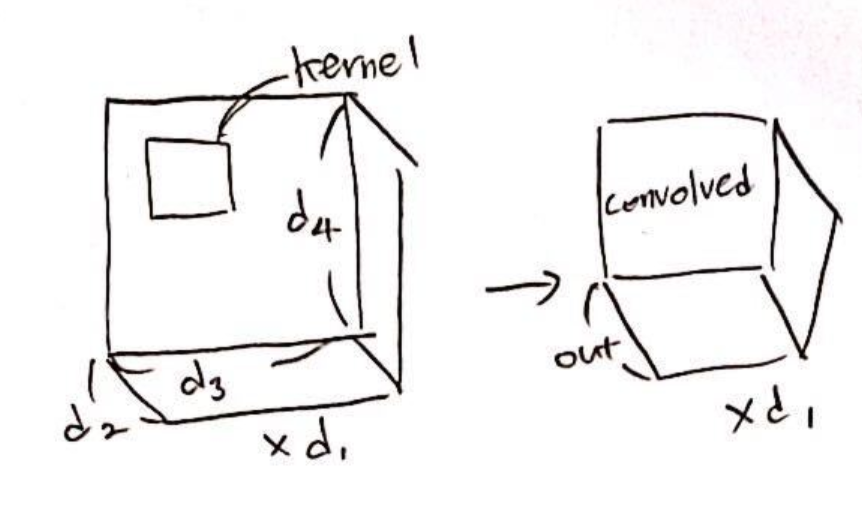
\includegraphics[height=12em]{resources/conv2d.png}
}{
  \begin{itemizec}
    \item $input\_size, hidden\_size, num\_layers > 0$
    \item Let $num\_directions \triangleq \ifs{bidirectional}{2}{1}$
    \item $\op{rank}{|input|} = \op{rank}{|hidden|} = 3$
    \item If $batch\_first == False$ then
    \begin{itemize}
      \item $|input| = (d_1, N, input\_size)$
    \end{itemize}
    \item If $batch\_first == True$ then
    \begin{itemize}
      \item $|input| = (N, d_2, input\_size)$
    \end{itemize}
    \item $|hidden| = (num\_layers \x num\_directions, N, hidden\_size)$
  \end{itemizec}
}{
  \begin{itemizec}
    \item 2-tuple of $(y, z)$ s.t.
    \begin{itemize}
      \item $|y| = |input| \indr{1}{2} \conc (num\_directions \x hidden\_size)$
      \item $|z| = |hidden|$
    \end{itemize}
  \end{itemizec}
}{
  \begin{itemizec}
    \item 간단한 recurrent 레이어입니다.
    \item 입력 텐서의 브로드캐스팅 적용 안 되고 무조건 rank-3여야 합니다.
    \item $hidden$ 텐서 shape의 constraint는 $batch\_first$ 변수와 무관함
  \end{itemizec}
}
\begin{align*}
  \frac
  {
    \begin{array}{l}
      \sigma \vdash E \Rar e, c_e \\
      \sigma \vdash H \Rar h, c_h \\
      c_{dim} = \{(input\_size, hidden\_size, num\_layers > 0) \land (\op{rank}{e} = 3)
        \land (\op{rank}{h} = 3)\} \\
      num\_directions = \ifs{bidirectional}{2}{1} \\
      c_{input} = \{ (\ifs{batch\_first}{(e[1] = h[2])}{(e[2] = h[2])}) \} \\
      c_{hidden} = \{ (h[1] = num\_layers \x num\_directions) \land
        (h[3] = hidden\_size) \} \\
      e' = e\indr{1}{2} \conc (num\_directions \x hidden\_size)
    \end{array}
  }
  {
    \sigma \vdash \module{RNN}{input\_size, hidden\_size, num\_layers=1,
      ..., bidirectional=False}{E, H} \Rar (e', h), c_e \cup c_h \cup c_{dim}
      \cup c_{input} \cup c_{hidden}
  } \\
  \\
  \text{텐서 2개(output, changed hidden states)를 묶은 2-tuple 형태로 반환}
\end{align*}


\subsection*{\ttt{torch.nn.LSTM}}
\prepostc{torch.nn.LSTM(input\_size, hidden\_size, num\_layers=1,
bias=True, batch\_first=False, dropout=0,
bidirectional=False)(input, (hidden, cell))}{
  %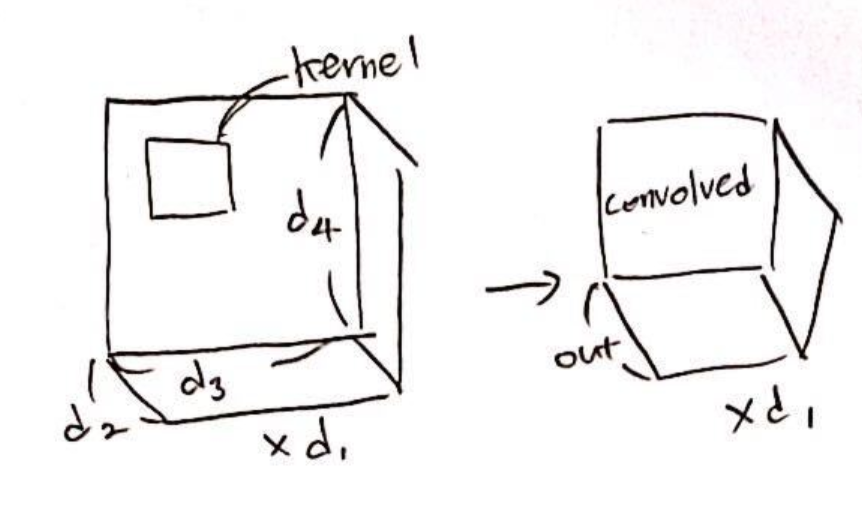
\includegraphics[height=12em]{resources/conv2d.png}
}{
  \begin{itemizec}
    \item $input\_size, hidden\_size, num\_layers > 0$
    \item Let $num\_directions \triangleq \ifs{bidirectional}{2}{1}$
    \item $\op{rank}{|input|} = \op{rank}{|hidden|} = \op{rank}{|cell|} = 3$
    \item If $batch\_first == False$ then
    \begin{itemize}
      \item $|input| = (d_1, N, input\_size)$
    \end{itemize}
    \item If $batch\_first == True$ then
    \begin{itemize}
      \item $|input| = (N, d_2, input\_size)$
    \end{itemize}
    \item $|hidden| = |cell|$
    \item[] $\bigspace = (num\_layers \x num\_directions, N, hidden\_size)$
  \end{itemizec}
}{
  \begin{itemizec}
    \item 2-tuple of $(y, (z, w))$ s.t., 
    \begin{itemize}
      \item $|y| = |input| \indr{1}{2} \conc (num\_directions \x hidden\_size)$
      \item $|z| = |w| = |hidden|$
    \end{itemize}
  \end{itemizec}
}{
  \begin{itemizec}
    \item Cell state도 추가적으로 가지는 LSTM 레이어입니다.
    \item $(hidden, cell)$을 왜 묶어서 표현했는지는 예제 코드를 보시면 명료하게 이해되실 겁니다.
  \end{itemizec}
}
\begin{align*}
  \frac
  {
    \begin{array}{l}
      \sigma \vdash E \Rar e, c_e \\
      \sigma \vdash H \Rar h, c_h \\
      \sigma \vdash L \Rar l, c_l \bigspace \text{(cell)} \\
      c_{dim} = \{(input\_size, hidden\_size, num\_layers > 0) \land (\op{rank}{e} = 3)
        \land (\op{rank}{h} = 3) \land (\op{rank}{l} = 3)\} \\
      num\_directions = \ifs{bidirectional}{2}{1} \\
      c_{input} = \{ (\ifs{batch\_first}{(e[1] = h[2])}{(e[2] = h[2])}) \} \\
      c_{hidden} = \{ (h[1] = num\_layers \x num\_directions) \land
        (h[3] = hidden\_size) \} \\
      c_{cell} = \{ (l[1] = num\_layers \x num\_directions) \land
        (l[3] = hidden\_size) \} \\
      e' = e\indr{1}{2} \conc (num\_directions \x hidden\_size)
    \end{array}
  }
  {
    \sigma \vdash \module{LSTM}{input\_size, hidden\_size, num\_layers=1,
      ..., bidirectional=False}{E, (H, L)} \Rar (e', (h, l)), c_e 
      \cup \cdots \cup c_{cell}
  } \\
  \\
  \text{예제 코드 참조 바랍니다.}
\end{align*}
Example Codes:
\begin{Verbatim}[tabsize=4,xleftmargin=2em]
lstm = torch.nn.LSTM(input_size=5, hidden_size=3, num_layers=4)
input = torch.randn(7, 6, 5)  # sequence length = 7, batch size = 6
hidden = torch.randn(4, 6, 3)
cell = torch.randn(4, 6, 3)

output, (hidden_out, cell_out) = lstm(input, (hidden, cell))
print(output.shape)           # (7, 6, 3)
print(hidden_out.shape)       # (4, 6, 3)
print(cell_out.shape)         # (4, 6, 3)
\end{Verbatim}


\subsection*{\ttt{torch.nn.GRU}}
\prepostc{torch.nn.GRU(input\_size, hidden\_size, num\_layers=1,
bias=True, batch\_first=False, dropout=0,
bidirectional=False)(input, hidden)}{
  %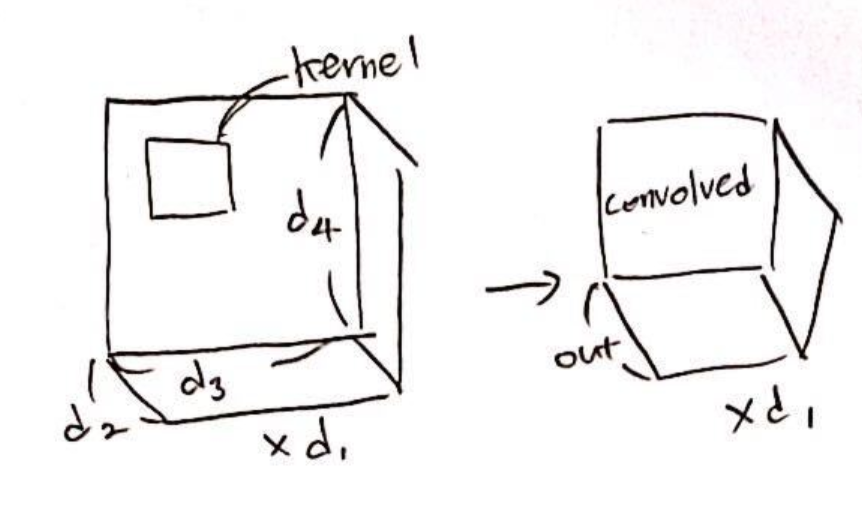
\includegraphics[height=12em]{resources/conv2d.png}
}{
  \begin{itemizec}
    \item $input\_size, hidden\_size, num\_layers > 0$
    \item Let $num\_directions \triangleq \ifs{bidirectional}{2}{1}$
    \item $\op{rank}{|input|} = \op{rank}{|hidden|} = 3$
    \item If $batch\_first == False$ then
    \begin{itemize}
      \item $|input| = (d_1, N, input\_size)$
    \end{itemize}
    \item If $batch\_first == True$ then
    \begin{itemize}
      \item $|input| = (N, d_2, input\_size)$
    \end{itemize}
    \item $|hidden| = (num\_layers \x num\_directions, N, hidden\_size)$
  \end{itemizec}
}{
  \begin{itemizec}
    \item 2-tuple of $(y, z)$ s.t.
    \begin{itemize}
      \item $|y| = |input| \indr{1}{2} \conc (num\_directions \x hidden\_size)$
      \item $|z| = |hidden|$
    \end{itemize}
  \end{itemizec}
}{
  \begin{itemizec}
    \item 비교적 최근에 나온 GRU 레이어입니다.
    \item RNN과 shape 연산이 비슷합니다.
  \end{itemizec}
}
\begin{align*}
  \frac
  {
    \begin{array}{l}
      \sigma \vdash E \Rar e, c_e \\
      \sigma \vdash H \Rar h, c_h \\
      c_{dim} = \{(input\_size, hidden\_size, num\_layers > 0) \land (\op{rank}{e} = 3)
        \land (\op{rank}{h} = 3)\} \\
      num\_directions = \ifs{bidirectional}{2}{1} \\
      c_{input} = \{ (\ifs{batch\_first}{(e[1] = h[2])}{(e[2] = h[2])}) \} \\
      c_{hidden} = \{ (h[1] = num\_layers \x num\_directions) \land
        (h[3] = hidden\_size) \} \\
      e' = e\indr{1}{2} \conc (num\_directions \x hidden\_size)
    \end{array}
  }
  {
    \sigma \vdash \module{GRU}{input\_size, hidden\_size, num\_layers=1,
      ..., bidirectional=False}{E, H} \Rar (e', h), c_e \cup c_h \cup c_{dim}
      \cup c_{input} \cup c_{hidden}
  } \\
  \\
  \text{텐서 2개(output, changed hidden states)를 묶은 2-tuple 형태로 반환}
\end{align*}




\section*{Embeddings}
\subsection*{\ttt{torch.nn.Embedding}}
\prepostc{torch.nn.Embedding(num\_embeddings, embedding\_dim, padding\_idx=None,
max\_norm=None, norm\_type=2.0, scale\_grad\_by\_freq=False,
sparse=False, \_weight=None)(input)}{
  %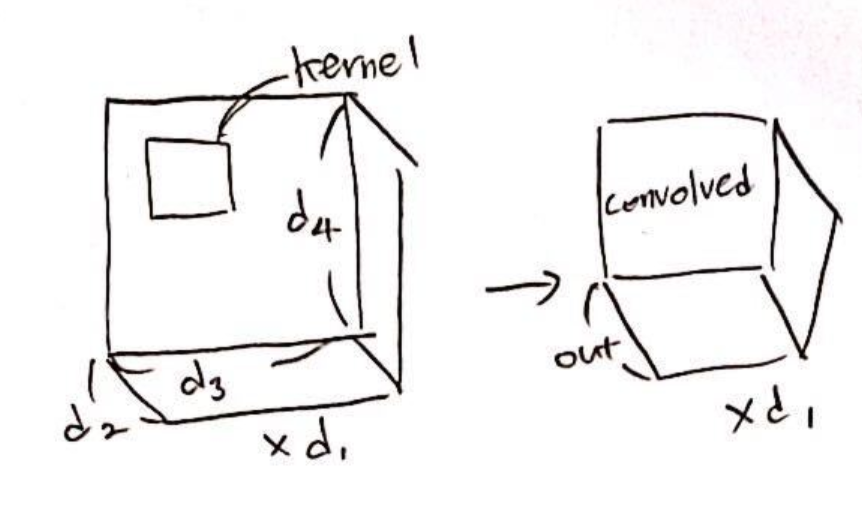
\includegraphics[height=12em]{resources/conv2d.png}
}{
  \begin{itemizec}
    \item $|input| = (d_1, d_2, \dots, d_k)$
    \item $\_weight$ is $None$ or
    \item[] $|\_weight| = (num\_embeddings, embedding\_dim)$
  \end{itemizec}
}{
  \begin{itemizec}
    \item $|y| = (d_1, d_2, \dots, d_k, embedding\_dim)$
  \end{itemizec}
}{
  \begin{itemizec}
    \item Input dimension이 너무 큰 경우를 효율적으로 처리하기 위한 row embedding
    \item $input$의 각 원소가 $num\_embeddings$보다 작아야한다는 constraint가
    있으나 shape 연산에는 영향을 주지 않음
  \end{itemizec}
}
\begin{align*}
  \frac
  {
    \begin{array}{l}
      \sigma \vdash E \Rar e, c \\
      \sigma \vdash \_weight \Rar w, c_w \bigspace\text{if $\_weight \neq None$} \\
      c_w = \{ (\_weight = None \lor w = (num\_embeddings, embedding\_dim)) \} \\
      e' = e \conc (embedding\_dim)
    \end{array}
  }
  {
    \sigma \vdash \module{Embedding}{num\_embedding, embedding\_dim, ..., \_weight=None}
    {E} \Rar e', c \cup c_w
  }
\end{align*}


\subsection*{\ttt{torch.nn.EmbeddingBag}}
\prepostc{torch.nn.EmbeddingBag(num\_embeddings, embedding\_dim, max\_norm=None,
norm\_type=2.0, scale\_grad\_by\_freq=False, mode=`mean', sparse=False,
\_weight=None, include\_last\_offset=False)(input, offset=None)}{
  %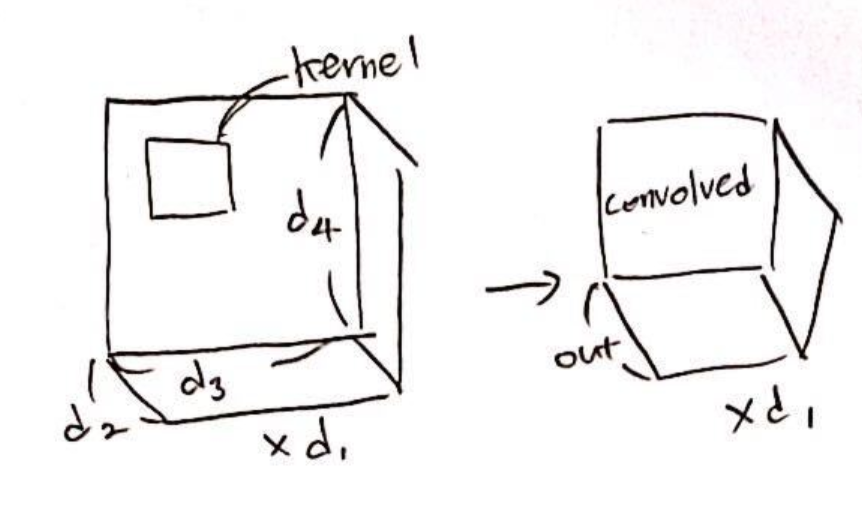
\includegraphics[height=12em]{resources/conv2d.png}
}{
  \begin{itemizec}
    \item $\op{rank}{|input|} \in \{1, 2\}$
    \item If $\op{rank}{|input|} = 1$ then
    \begin{itemize}
      \item $offset \neq None$ and $\op{rank}{|offset|} = 1$
    \end{itemize}
    \item If $\op{rank}{|input|} = 2$ then
    \begin{itemize}
      \item $offset = None$
    \end{itemize}
    \item $\_weight$ is $None$ or
    \item[] $|\_weight| = (num\_embeddings, embedding\_dim)$
  \end{itemizec}
}{
  \begin{itemizec}
    \item If $\op{rank}{|input|} = 1$ then
    \begin{itemize}
      \item $|y| = (|offset|[1], embedding\_dim)$
    \end{itemize}
    \item If $\op{rank}{|input|} = 2$ then
    \begin{itemize}
      \item $|y| = (|input|[1], embedding\_dim)$
    \end{itemize}
  \end{itemizec}
}{
  \begin{itemizec}
    \item 여러 sementic constraint가 있지만 shape에는 영향을 안 줌
    \item $input$ 텐서의 차원에 따라 기능이 달라지는 함수
  \end{itemizec}
}
\begin{align*}
  \frac
  {
    \begin{array}{l}
      \sigma \vdash E \Rar e, c \\
      \sigma \vdash \_weight \Rar w, c_w \bigspace\text{if $\_weight \neq None$} \\
      \sigma \vdash offset \Rar o, c_o \bigspace \text{if $offset \neq None$} \\
      c_w = \{ (\_weight = None \lor w = (num\_embeddings, embedding\_dim)) \} \\
      c_{dim} = \{ (\op{rank}{e} \in \{1,2\}) \land
        (\ifs{\op{rank}{e} = 1}{(offset \neq None \land \op{rank}{o} = 1)}
        {(offset = None)}) \} \\
      e' = \ifs{\op{rank}{e} = 1}{(o[1], embedding\_dim)}{(e[1], embedding\_dim)}
    \end{array}
  }
  {
    \sigma \vdash \module{EmbeddingBag}{num\_embedding, embedding\_dim, ...,
      include\_last\_offset=False}{E, offset=None} \Rar e', c \cup c_w \cup c_{dim}
  }
\end{align*}


\subsection*{(Builtin) \ttt{torch.nn.functional.embedding}}
\prepost{torch.nn.functional.embedding(input, weight, padding\_idx=None,
max\_norm=None, norm\_type=2.0, scale\_grad\_by\_freq=False, sparse=False)}{
  %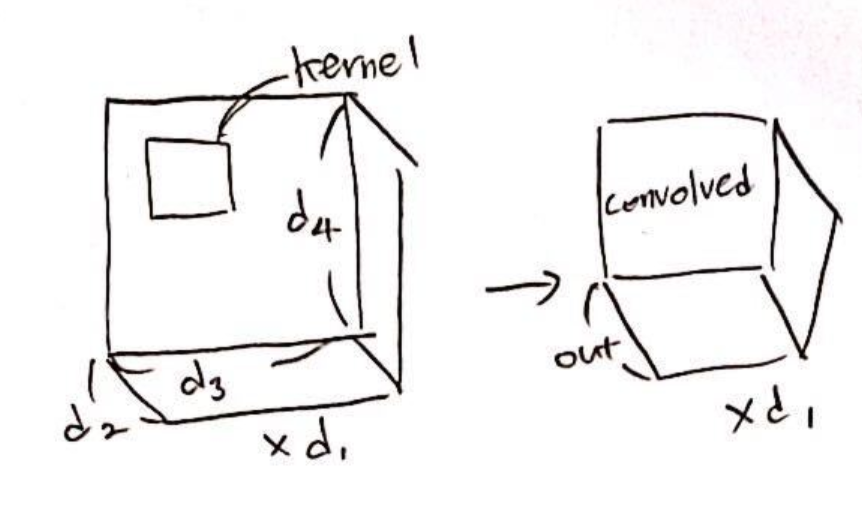
\includegraphics[height=12em]{resources/conv2d.png}
}{
  \begin{itemizec}
    \item $|input| = (d_1, d_2, \dots, d_k)$
    \item $|weight| = (w_1, w_2)$
  \end{itemizec}
}{
  \begin{itemizec}
    \item $|y| = (d_1, d_2, \dots, d_k, w_2)$
  \end{itemizec}
}
\begin{align*}
  \frac
  {
    \begin{array}{l}
      \sigma \vdash E \Rar e, c_e \\
      \sigma \vdash W \Rar w, c_w \\
      c_{dim} = \{ (\op{rank}{w} = 2) \} \\
      e' = e \conc (w[2])
    \end{array}
  }
  {
    \sigma \vdash \op{embedding}{E, W, padding\_idx=None, ..., sparse=False}
      \Rar e', c_e \cup c_w \cup c_{dim}
  }
\end{align*}




\end{document}
